\chapter{Cwiczenie 2}

\section{Krzywe Lissajous}

Korzystając z trybu \textbf{X-Y} oscyloskopu zaobserwowano efekt złożenia dwóch drgań harmonicznych (\textbf{krzywe Lissajous})

\begin{itemize}
    \item Włączono \textbf{tryb X-Y}
    \item Wysłano \textbf{sygnały sinusoidalne} na oba kanały \textcolor{purple}{(o amplitudzie \textbf{1V} oraz bazowej częstotliwości \textbf{15kHz} (w proporcji \textbf{1} oznacza \textbf{15kHz}))}
    \label{ad:dodatkowe_informacje_lissajous}
    \item Ustawiono sygnały w stosunku kolejno: \textbf{1:1, 1:2, 1:3} (częstotliwość) oraz przesunięciu fazowym \textbf{90}\boldsymbol{\degree} ($\frac{\pi}{2}$)
\end{itemize}

\label{ad:teoretyczne_lissajous}
{
    \begin{figure}[H]
        \centering
        \begin{subfigure}[h]{0.45\textwidth}
            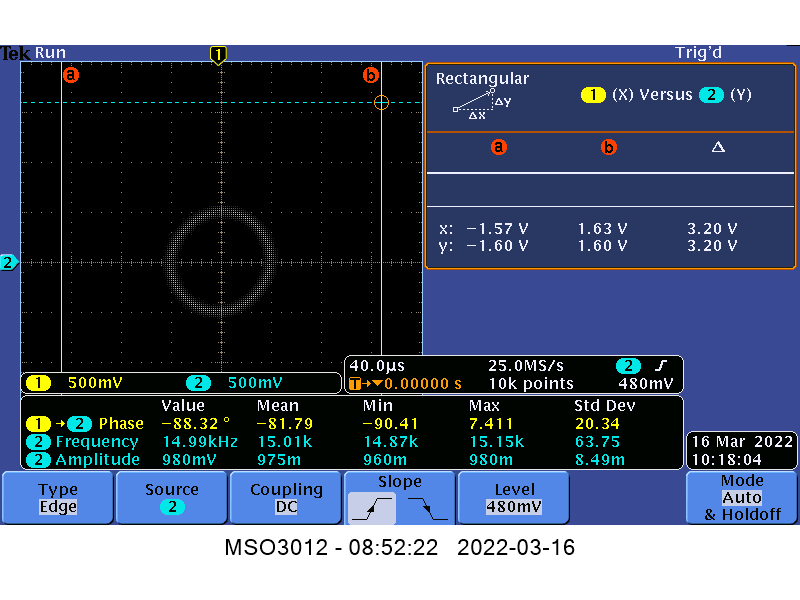
\includegraphics[scale=0.3]{images/1_5_1-1-90.png}
            \caption*{1:1 90$\degree$}
        \end{subfigure}
        \begin{subfigure}[h]{0.45\textwidth}
            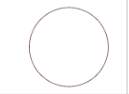
\includegraphics[scale=1.9]{images/theoretical/1-1-90.png}
            \caption*{1:1 90$\degree$ teoretyczna}
        \end{subfigure}
    \end{figure}
    
    \begin{figure}[H]
        \centering
        \begin{subfigure}[h]{0.45\textwidth}
            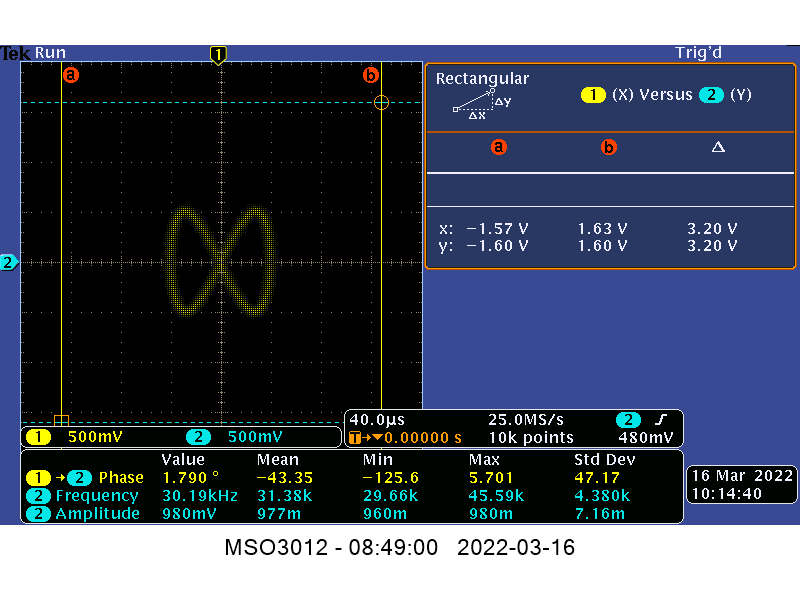
\includegraphics[scale=0.3]{images/1_5_1-2-90.png}
            \caption*{1:2 90$\degree$}
        \end{subfigure}
        \begin{subfigure}[h]{0.45\textwidth}
            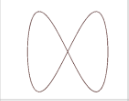
\includegraphics[scale=1.9]{images/theoretical/1-2-90.png}
            \caption*{1:2 90$\degree$ teoretyczna}
        \end{subfigure}
    \end{figure}
    
    \begin{figure}[H]
        \centering
        \begin{subfigure}[h]{0.45\textwidth}
            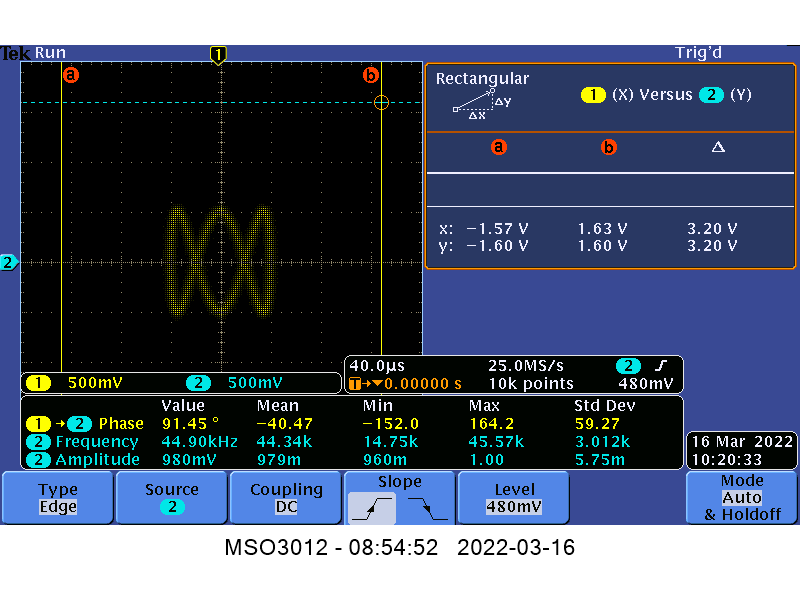
\includegraphics[scale=0.3]{images/1_5_1-3-90.png}
            \caption*{1:3 90$\degree$}
        \end{subfigure}
        \begin{subfigure}[h]{0.45\textwidth}
            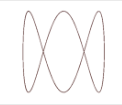
\includegraphics[scale=1.9]{images/theoretical/1-3-90.png}
            \caption*{1:3 90$\degree$ teoretyczna}
        \end{subfigure}
    \end{figure}
}

\begin{itemize}
    \item Następnie ustawiono sygnały w stosunku kolejno: \textbf{1:1, 1:3} (częstotliwość) oraz przesunięciu fazowym \textbf{45}\boldsymbol{\degree} ($\frac{\pi}{4}$)
{
    \begin{figure}[H]
        \centering
        \begin{subfigure}[h]{0.45\textwidth}
            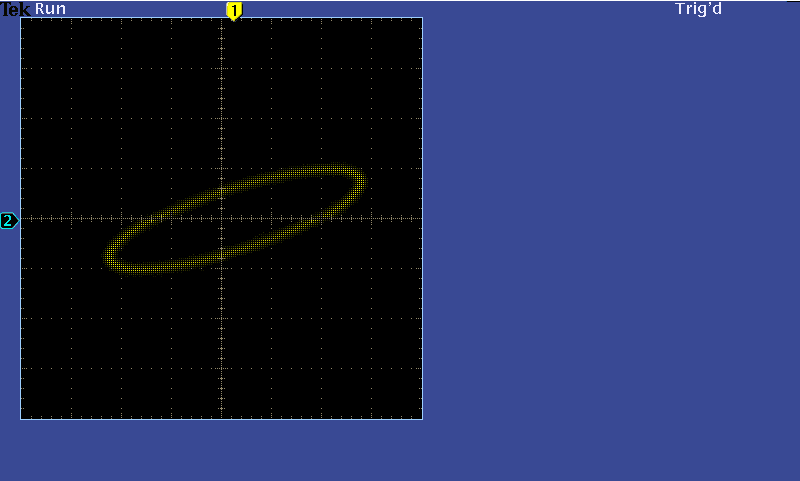
\includegraphics[scale=0.3]{images/zad.5.2.png}
            \caption*{1:1 45$\degree$}
        \end{subfigure}
        \begin{subfigure}[h]{0.45\textwidth}
            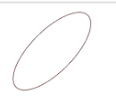
\includegraphics[scale=1.9]{images/theoretical/1-1-45.png}
            \caption*{1:1 45$\degree$ teoretyczna}
        \end{subfigure}
    \end{figure}
    
    \begin{figure}[H]
        \centering
        \begin{subfigure}[h]{0.45\textwidth}
            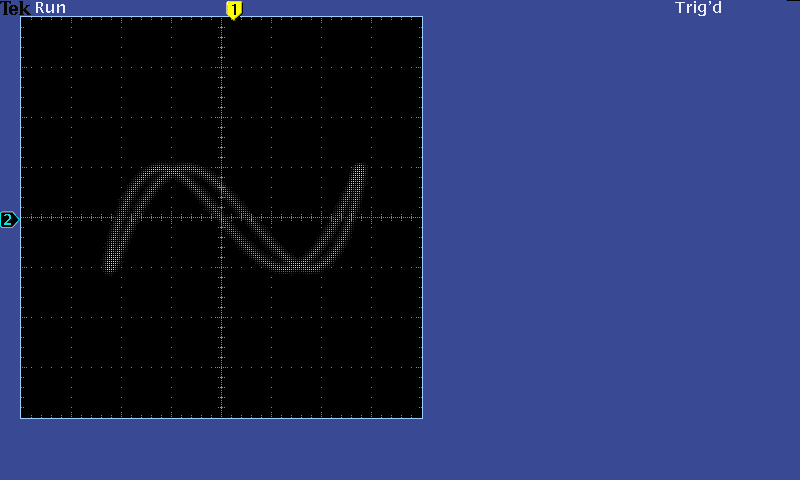
\includegraphics[scale=0.3]{images/zad.5.1.png}
            \caption*{1:3 45$\degree$}
        \end{subfigure}
        \begin{subfigure}[h]{0.45\textwidth}
            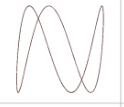
\includegraphics[scale=1.9]{images/theoretical/1-3-45.png}
            \caption*{1:3 45$\degree$ teoretyczna}
        \end{subfigure}
    \end{figure}
}

\end{itemize}